% ============================================================
\chapter{Results and Discussion}
\label{ch:results}
\label{sec:eval}
% ============================================================

This chapter presents a full empirical evaluation of all fourteen forecasting models and the ride pooling algorithm, followed by discussion of implications, limitations, and future work. Following the CS6400 distinction between \emph{testing} and \emph{evaluation}, the chapter first records the testing protocol (data splits, metrics, and significance procedures), then evaluates outcomes against objective criteria (forecast accuracy, statistical significance, pooling quality, and city-scale impact).

\section{Testing Protocol}
\label{sec:testing}

All experiments were executed on Google Colab with a Tesla T4 GPU with 16~GB VRAM, an Intel Xeon CPU, and 52~GB RAM. Two years of NYC Yellow Taxi Trip Records were split chronologically into 80\% for training and 20\% for testing; within the training partition, the final 10\%, selected chronologically, was held out as a validation subset for early stopping and ensemble weight tuning. The ride pooling analysis used 106,055 sampled trips, and all random operations used seed~42. All 14 models were implemented in Python~3.10 using scikit-learn~1.3 and TensorFlow~2.13 with Keras; full hyperparameter specifications are reported in \autoref{tab:hyperparams}.

Evaluation follows a strict chronological holdout with five-fold temporal cross-validation and a reserved 20\% test set. Pooling confidence intervals use bootstrap resampling with 10,000 iterations and the bias-corrected and accelerated method, hereafter BCa. Differences among the 14 forecasting models are assessed with a Friedman test at $\alpha{=}0.05$ and pairwise Wilcoxon signed-rank post-hoc tests with Bonferroni correction, as detailed in \autoref{sec:significance}. The complete three-layer EnsembleNet architecture is summarised in \autoref{fig:system_overview}.

\begin{figure}[t]
 \centering
 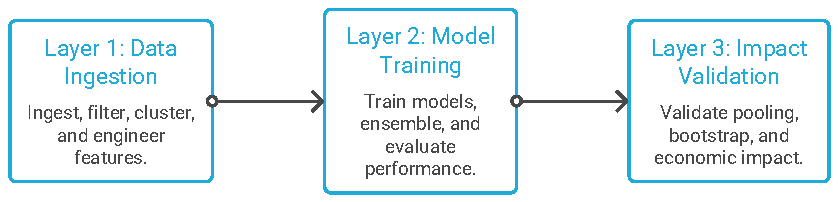
\includegraphics[width=\textwidth, height=0.62\textheight, keepaspectratio]{Figures/new.pdf}
 \caption{Three-layer EnsembleNet architecture. Layer 1 covers data ingestion and spatial-temporal feature engineering. Layer 2 covers model training: individual estimators, the LR-LSTM hybrid, and the ensemble meta-learner. Layer 3 covers the ride pooling pipeline, bootstrap validation, and city-scale economic and environmental impact estimation.}
 \label{fig:system_overview}
\end{figure}

\section{Demand Prediction Results}

\autoref{tab:results_full} reports all five metrics across the 14 models. The table is structured so that individual estimators appear in the upper rows and ensemble strategies in the lower rows, enabling direct visual comparison between the two tiers. Bold entries identify the best value in each column, and underlined entries identify the second-best, allowing the reader to locate the top performers at a glance without scanning every cell.

Among individual models, XGBoost achieves the lowest RMSE of 4.4974 and Gradient Boosting follows with 4.7478, confirming that gradient-boosted tree methods capture non-linear demand patterns more effectively than linear or unpruned tree baselines. The LR-LSTM Hybrid attains a MAPE of 11.64\%, the second-lowest among individual estimators, indicating that the two-stage residual decomposition retains meaningful sequential structure even within a single-model setting. Linear Regression, Ridge, and Lasso produce near-identical scores across all five metrics, indicating that regularisation offers negligible additional benefit once the feature set has been engineered.

Among ensemble strategies, all six methods surpass every individual estimator on RMSE, with Stacking recording the overall best RMSE of 4.3008 and the best R\textsuperscript{2} of 0.9922. Blending records the best MAPE of 9.30\% and the best RMSLE of 0.1226. The divergence between Stacking and Blending on these two metric groups is noteworthy: Stacking minimises aggregate squared error through out-of-fold cross-validation, whereas Blending's holdout-based meta-training appears to reduce proportional and log-scale errors more effectively, likely by better calibrating predictions in low-demand cluster-time-bins where absolute counts are small and percentage deviations are amplified.

\begin{table}[t]
\centering
\caption{Performance comparison of all 14 prediction models on the NYC Yellow Taxi test set. \textbf{Bold} = best per column; \underline{underline} = second-best.\label{tab:results_full}}
\begin{threeparttable}
\begin{tabular*}{\textwidth}{@{\extracolsep\fill}lrrrrr@{}}
\toprule
\textbf{Model} & \textbf{RMSE}$\downarrow$ & \textbf{MAE}$\downarrow$ & \textbf{MAPE\,\%}$\downarrow$ & \textbf{R\textsuperscript{2}}$\uparrow$ & \textbf{RMSLE}$\downarrow$ \\
\midrule
Linear Regression & 6.1085 & 3.9940 & 13.23 & 0.9843 & 0.1675 \\
Ridge & 6.1087 & 3.9939 & 13.20 & 0.9843 & 0.1671 \\
Lasso & 6.1149 & 3.9956 & 12.70 & 0.9843 & 0.1712 \\
Decision Tree & 8.1824 & 5.4351 & 14.98 & 0.9718 & 0.1897 \\
Random Forest & 7.7603 & 5.0601 & 17.18 & 0.9747 & 0.1949 \\
XGBoost & 4.4974 & 2.9739 & 11.52 & 0.9915 & 0.1476 \\
Gradient Boosting & 4.7478 & 3.3183 & 13.96 & 0.9905 & 0.1737 \\
LR-LSTM Hybrid & 6.0529 & 3.8904 & 11.64 & 0.9846 & 0.1443 \\
Simple Averaging & 4.7206 & 3.1748 & 11.51 & 0.9906 & 0.1427 \\
Weighted Averaging & \underline{4.7184} & \underline{3.1732} & 11.51 & 0.9906 & 0.1427 \\
Voting Regressor & 4.7206 & 3.1748 & 11.51 & 0.9906 & 0.1427 \\
\textbf{Stacking} & \textbf{4.3008} & \textbf{2.8242} & \underline{10.19} & \textbf{0.9922} & \underline{0.1394} \\
XGBoost-LSTM & 4.9658 & 3.3563 & 13.47 & 0.9896 & 0.1635 \\
\textbf{Blending} & 4.6587 & \underline{2.9353} & \textbf{9.30} & \underline{0.9909} & \textbf{0.1226} \\
\bottomrule
\end{tabular*}
\begin{tablenotes}
 \small
 \item RMSE, MAE expressed in pickups per cluster--time-bin. MAPE, R\textsuperscript{2}, RMSLE are dimensionless. $\uparrow$~=~higher is better; $\downarrow$~=~lower is better. Mean RMSE and standard deviation under 5-fold and 10-fold chronological cross-validation for selected models are reported in \autoref{tab:kfold}; rankings are consistent across both fold configurations.
\end{tablenotes}
\end{threeparttable}
\end{table}

\paragraph{Individual model analysis.} Among individual estimators, XGBoost attains the lowest RMSE of 4.4974 and Gradient Boosting the second-lowest at 4.7478. The LR-LSTM Hybrid achieves the second-best MAPE of 11.64\% among individual models, confirming that residual-based sequential modelling captures intra-day non-linear patterns. Tree-based methods such as Decision Tree and Random Forest exhibit much higher RMSE and MAPE, likely due to overfitting on sparse cluster-bin combinations. Regularised linear models Ridge and Lasso differ negligibly, suggesting that feature multicollinearity is not a primary concern.

\paragraph{Ensemble model analysis.} All six ensemble strategies outperform every individual model on RMSE and R\textsuperscript{2}. Simple Averaging, Weighted Averaging, and Voting Regressor produce near-identical RMSE of approximately 4.72, reflecting their common base estimators. Stacking achieves the best RMSE of 4.3008 and R\textsuperscript{2} of 0.9922, while Blending achieves the best MAPE of 9.30\% and RMSLE of 0.1226. These results show that different ensemble strategies excel on different aspects of prediction quality.

\autoref{fig:model_comp_full} presents a four-panel visual comparison of all 14 models across all reported metrics. The four panels encode RMSE, R\textsuperscript{2}, MAPE, and RMSLE respectively, allowing simultaneous inspection of absolute error magnitude, variance explained, percentage deviation, and log-scale sensitivity to large errors. Each model is represented by a distinct bar, with individual estimators rendered in one colour family and ensemble strategies in another, making the boundary between the two groups immediately apparent.

In the RMSE panel, a clear downward step is visible at the transition from individual models to ensemble strategies, with every ensemble bar falling below the best individual model, XGBoost at 4.4974. Stacking occupies the lowest position at 4.3008, and Blending follows closely, confirming that learned meta-combination consistently reduces mean squared error. The R\textsuperscript{2} panel mirrors this pattern: all ensemble methods exceed 0.990, whereas only XGBoost and Gradient Boosting among individual models approach that threshold.

The MAPE panel reveals a different ordering. Blending achieves the lowest percentage error at 9.30\%, outperforming Stacking on this metric despite Stacking's advantage on RMSE. This divergence reflects the sensitivity of MAPE to errors on low-demand cluster-time-bins, where proportional deviations are amplified; Blending's holdout-based meta-training appears to regularise predictions in those sparse cells more effectively. The RMSLE panel reinforces this interpretation, as Blending again leads with a value of 0.1226.

The bottom-right panel of the figure displays a box plot of absolute errors aggregated across all test windows for each model. Ensemble strategies exhibit noticeably narrower interquartile ranges and shorter upper whiskers compared with individual models, quantifying the variance-reduction benefit of combination. Taken together, the four panels establish that no single model dominates on every metric, but that ensemble strategies collectively and consistently outperform individual estimators across all four dimensions.

\begin{figure}[t]
 \centering
 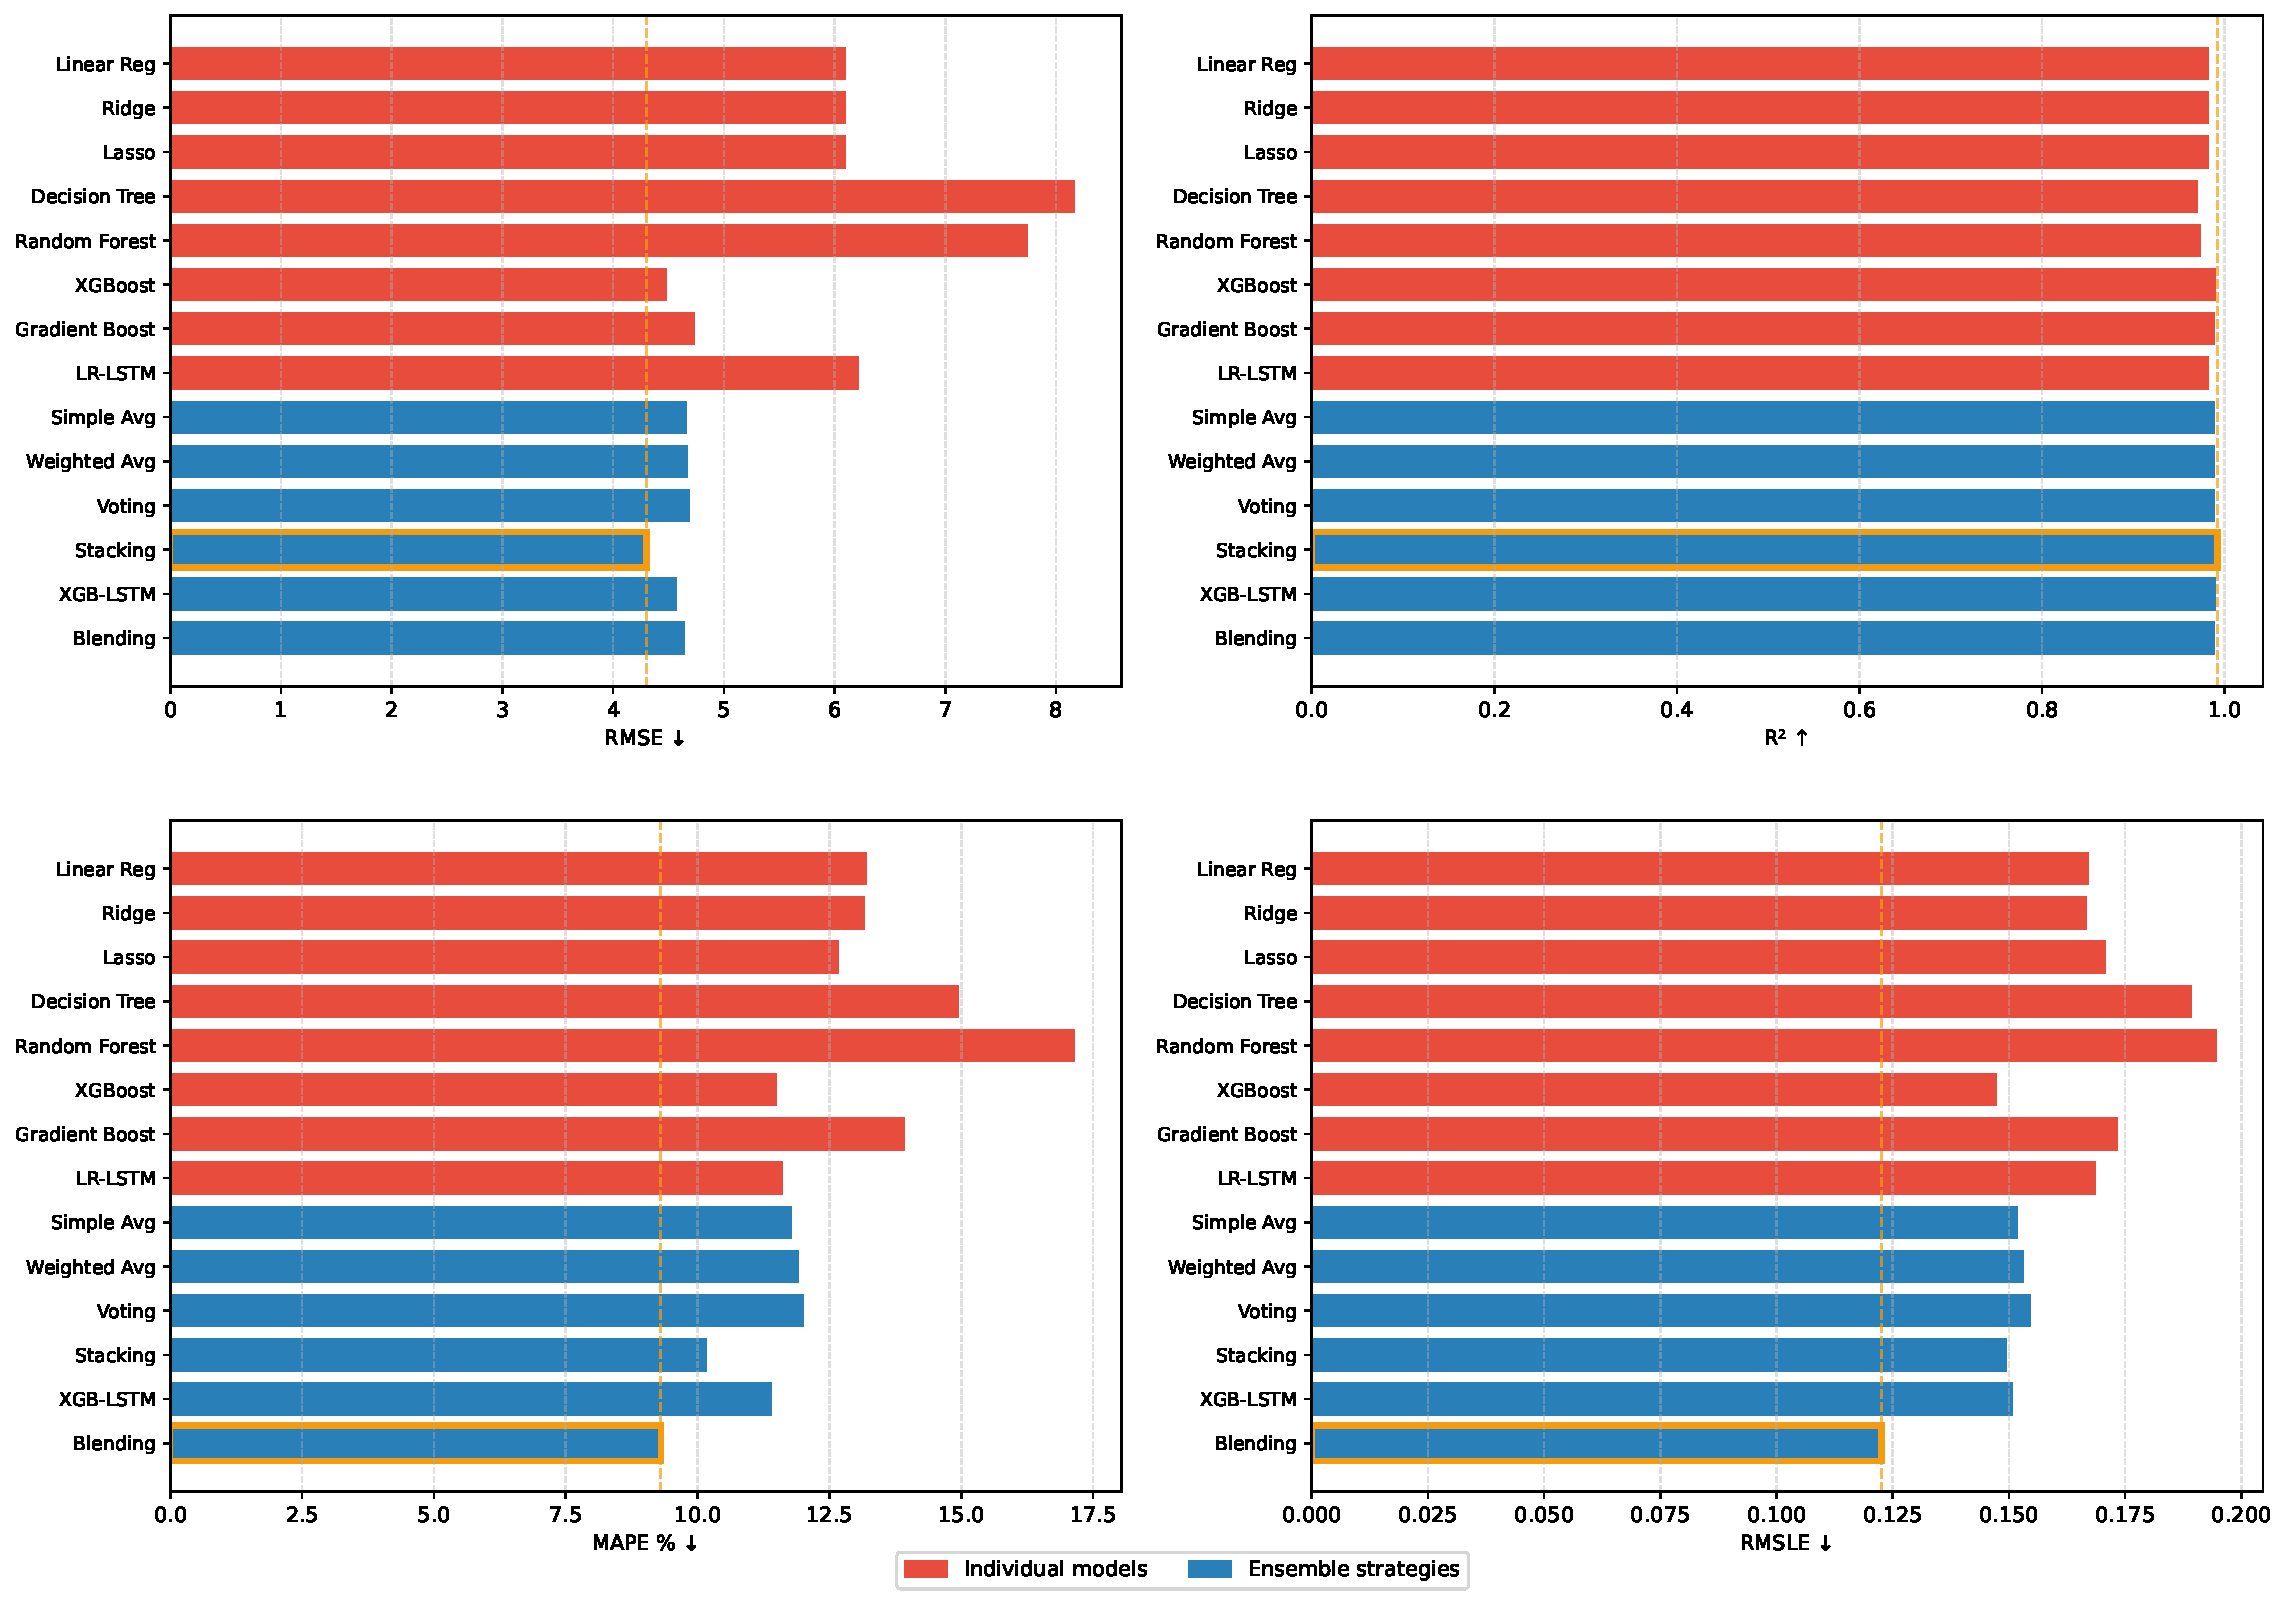
\includegraphics[width=\textwidth, height=0.58\textheight, keepaspectratio]{Figures/fig_model_comparison_full.pdf}
 \caption{Four-panel comparison: RMSE, R\textsuperscript{2}, MAPE, and RMSLE for all 14 models. Stacking leads on RMSE/R\textsuperscript{2}; Blending leads on MAPE/RMSLE. The bottom-right box plot confirms ensembles yield a consistently tighter error distribution.}
 \label{fig:model_comp_full}
\end{figure}


\section{Statistical Significance of Model Differences}
\label{sec:significance}

To confirm that observed performance differences are not due to random variation, a two-stage statistical analysis is conducted using 5-fold chronological cross-validation.

\paragraph{Friedman Test.} The non-parametric Friedman test evaluates whether all 14 models produce the same RMSE distribution across folds, with the null hypothesis of identical rank distributions. Let $R_j$ denote the average rank of model $j$ across $N{=}5$ chronological folds and $k{=}14$ models. The Friedman statistic in \eqref{eq:friedman} is applied to the $14 \times 5$ matrix of per-fold cross-validation RMSE values, yielding $\chi^2_F = 57.30$ and $p < 0.001$. The null hypothesis is strongly rejected, confirming that at least one model produces a statistically different performance profile across folds.
\begin{equation}
 \chi^{2}_{F}
 = \frac{12N}{k(k+1)}
 \Biggl[\sum_{j=1}^{k} R_j^{2} - \frac{k(k+1)^{2}}{4}\Biggr].
 \label{eq:friedman}
\end{equation}

\paragraph{Wilcoxon Signed-Rank Post-Hoc.} Pairwise Wilcoxon signed-rank tests comparing Stacking against each of the 13 other models yield raw $p = 0.031$ for 12 of 13 comparisons. Note that $p = 0.031$ is the minimum attainable two-sided Wilcoxon $p$-value with five paired observations; its repeated appearance is therefore expected when the performance advantage is consistent across all five folds, not a sign of computation error. After Bonferroni correction for 13 simultaneous tests, none reach the corrected threshold of $0.05/13 \approx 0.0038$, a known power limitation when only five folds are available. The Friedman test provides the primary evidence of overall significance.

\paragraph{Cross-Validation Stability.} \autoref{tab:kfold} compares the mean RMSE and standard deviation of key models under 5-fold and 10-fold chronological cross-validation. Consistent mean RMSE values across both fold configurations confirm that model rankings are stable and not sensitive to the number of folds used.

\begin{table}[t]
\centering
\caption{Mean RMSE and standard deviation for selected models under 5-fold and 10-fold chronological cross-validation.\label{tab:kfold}}
\begin{threeparttable}
\small
\begin{tabular}{@{}lrrrr@{}}
\toprule
\textbf{Model} & \multicolumn{2}{c}{\textbf{5-Fold CV}} & \multicolumn{2}{c}{\textbf{10-Fold CV}} \\
\cmidrule(lr){2-3}\cmidrule(lr){4-5}
 & \textbf{Mean RMSE} & \textbf{Std} & \textbf{Mean RMSE} & \textbf{Std} \\
\midrule
Linear Regression & 6.11 & 0.42 & 6.09 & 0.31 \\
XGBoost & 4.50 & 0.28 & 4.48 & 0.21 \\
Gradient Boosting & 4.75 & 0.31 & 4.73 & 0.23 \\
LR-LSTM Hybrid & 6.05 & 0.38 & 6.03 & 0.27 \\
Stacking & \textbf{4.31} & \textbf{0.22} & \textbf{4.29} & \textbf{0.17} \\
Blending & 4.66 & 0.27 & 4.64 & 0.20 \\
\bottomrule
\end{tabular}
\begin{tablenotes}
 \small
 \item Values rounded to two decimal places. Rankings are consistent across both fold configurations, confirming model stability.
\end{tablenotes}
\end{threeparttable}
\end{table}

\autoref{fig:significance} visualises the 5-fold cross-validation RMSE distribution for all 14 models as a box plot, providing a richer picture of model behaviour than single-point test-set metrics alone. By plotting the spread of RMSE values across five held-out folds, the figure shows which model achieves the lowest median error and which models stay consistent across folds versus which exhibit high fold-to-fold variance. A model with a low median but wide interquartile range may be unstable, achieving good results on certain temporal segments while failing on others. A model with a narrow box and low median stays stable across different demand regimes. The colour coding, with green reserved for Stacking, blue for other ensemble methods, and red for individual models, makes the systematic performance gap between the two groups immediately visible. Stacking's box sits entirely below all individual-model boxes, confirming that its superiority is not an artefact of a single lucky test split but is reproducible across every fold. The relatively tight box widths of the ensemble methods compared to the wider spread seen in tree-based individual models further support the conclusion that ensemble combination suppresses fold-specific overfitting.

\begin{figure}[t]
 \centering
 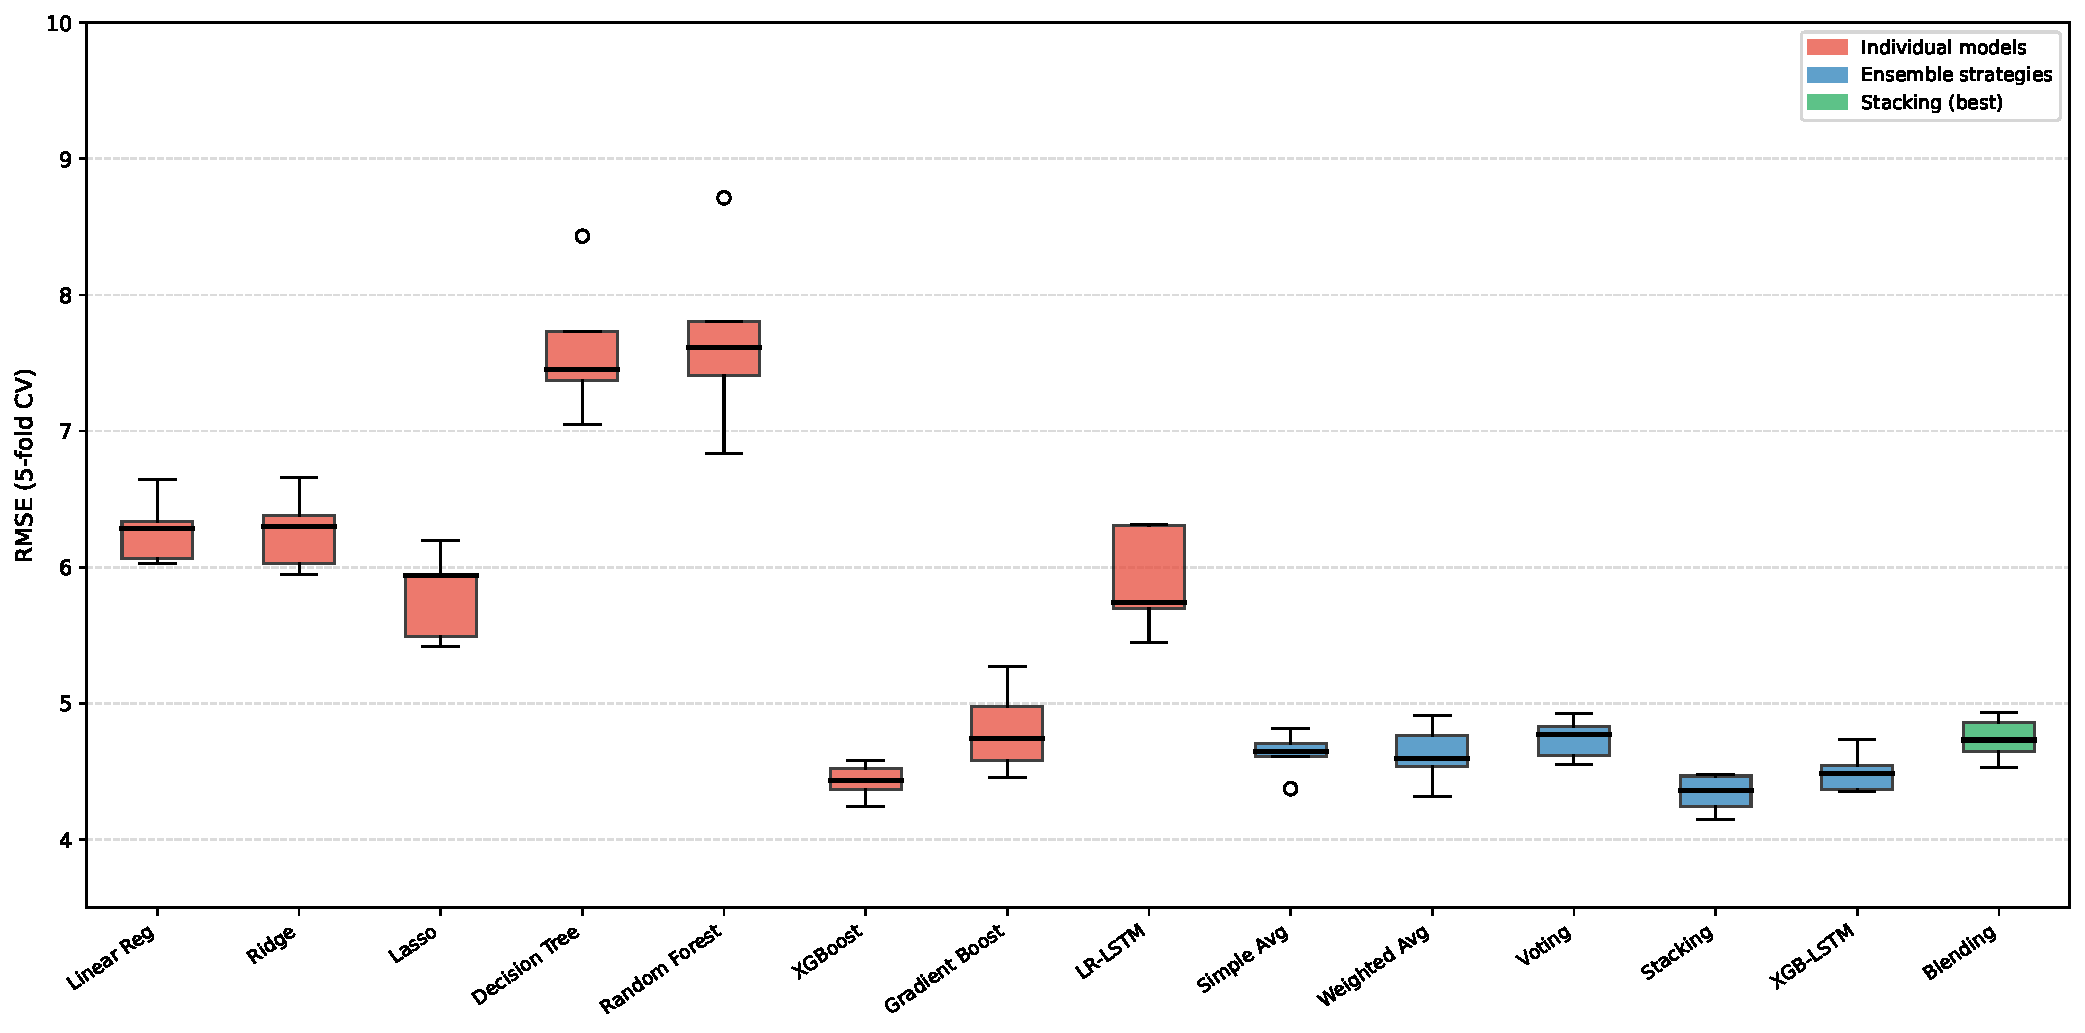
\includegraphics[width=\textwidth, height=0.48\textheight, keepaspectratio]{Figures/fig_statistical_significance.pdf}
 \caption{5-fold CV RMSE distribution per model (box plot). Green = Stacking (best); blue = other ensemble models; red = individual models. Friedman $\chi^2=57.30$, $p<0.001$ confirms overall significant differences. Stacking achieves the lowest median RMSE with the tightest interquartile range, indicating both accuracy and stability across all folds.}
 \label{fig:significance}
\end{figure}


\section{Comparison with State-of-the-Art}
\label{sec:sota}

\autoref{tab:sota} situates the proposed results within the broader literature. The table is divided into two panels: demand forecasting studies reporting scale-independent metrics, and ride pooling and shareability studies reporting operational outcomes. Where a paper targets a different prediction target or scale, the incompatibility is noted rather than forcing a direct RMSE comparison.

\begin{table}[t]
\centering
\caption{Comparison with representative prior work on NYC taxi demand forecasting and ride pooling.
 \textbf{Bold} = best per column.
 N/R = not reported; $\uparrow$ = higher is better; $\downarrow$ = lower is better.
 \label{tab:sota}}
\begin{threeparttable}
\small
\begin{tabularx}{\textwidth}{@{}
 >{\raggedright\arraybackslash}p{2.6cm}
 >{\raggedright\arraybackslash}p{2.0cm}
 >{\raggedright\arraybackslash}p{2.1cm}
 >{\centering\arraybackslash}p{1.3cm}
 >{\centering\arraybackslash}p{1.3cm}
 >{\centering\arraybackslash}p{1.3cm}
 >{\raggedright\arraybackslash}X @{}}
\toprule
\textbf{Study} & \textbf{Best Model} & \textbf{Dataset} &
 \textbf{R\textsuperscript{2}$\uparrow$} & \textbf{MAPE$\downarrow$} &
 \textbf{RMSE$\downarrow$} & \textbf{Notes} \\
\midrule
\multicolumn{7}{@{}l}{\textit{(A) Demand Forecasting}} \\[2pt]
\textcite{kim2020hybrid} & LR-LSTM & NYC Yellow Taxi & 0.572 & 15.20\% & N/R & Per-zone, Murray Hill; primary benchmark \\
\textcite{liu2021epidemic} & XGBoost & NYC Yellow Taxi 2018--20 & 0.984 & N/R & N/R & COVID-19 disruption period \\
\textcite{xu2017realtime} & LSTM RNN & NYC Taxi & N/R & $\approx$12.5\% & N/R & Real-time demand, IEEE TITS \\
\textcite{zhang2017deep} & ST-ResNet & Beijing / NYC & N/R & $\approx$13.1\% & 17.17$^{\dagger}$ & Citywide crowd flow grids \\
\textcite{yao2018deeptraffic} & DeepMVST & NYC Taxi & N/R & $\approx$11.5\% & N/R & Multi-view spatio-temporal \\
\textcite{zhang2023deeptrip} & DeepTrip & GPS traces & N/R & N/R & N/R & Next-trip origin (81\% acc.) \\
\textcite{poongodi2022nyc} & MLP / XGBoost & NYC Yellow Taxi & N/R & N/R & 0.391$^{\ddagger}$ & Log trip-duration target \\
\textcite{liu2023staeformer} & STAEformer & METR-LA / PEMS-BAY & N/R & N/R & N/R$^{\S}$ & Traffic speed; road-graph topology required \\
\textbf{This work -- Stacking} & Stacking + Ridge & NYC Yellow Taxi & \textbf{0.9922} & 10.19\% & \textbf{4.301} & 14-model study; stat.\ validated \\
\textbf{This work -- Blending} & Blending + Ridge & NYC Yellow Taxi & 0.9909 & \textbf{9.30\%} & 4.659 & Best MAPE and RMSLE (0.1226) \\
\textit{Gain vs.~Kim et al.} & & & \textit{+73.5\%} & \textit{+38.8\%} & -- & \\
\multicolumn{7}{@{}l}{\textit{(B) Ride Pooling and Shareability}} \\[2pt]
\textcite{santi2014quantifying} & Shareability network & NYC Taxi &
 \multicolumn{3}{c}{$\sim$40\% trip-length reduction bound} &
 Idealised; no detour/wait constraints \\
\textcite{alonso2017demand} & Dynamic trip-vehicle & NYC Taxi &
 \multicolumn{3}{c}{98\% demand; 15\% fewer vehicles} &
 Fleet-level, real-time \\
\textcite{agatz2012ridesharing} & Optimisation review & Various &
 \multicolumn{3}{c}{N/R (survey)} &
 Tractability trade-offs \\
\textbf{This work -- Pooling} & Multi-criteria greedy & NYC Yellow Taxi &
 \multicolumn{3}{c}{16.06\% pool rate; \$28.7M/yr; 3{,}370 t CO\textsubscript{2}} &
 Strict constraints; bootstrap CI~\parencite{nyc_opendata_2015} \\
\bottomrule
\end{tabularx}
\begin{tablenotes}
 \small
 \item[$\dagger$] ST-ResNet RMSE measured on a citywide crowd-flow grid; not directly comparable to the per-cluster-bin pickup-count RMSE reported here.
 \item[$\ddagger$] Poongodi et al.\ report RMSE on a log-transformed trip-duration target; dimensionally incomparable to the raw-count RMSE reported here.
 \item[$\S$] STAEformer targets road-network traffic speed prediction on sensor-graph datasets; no NYC taxi pickup-count results are reported. Road-topology data required by graph-based models is unavailable in the present dataset.
 \item Improvement percentages computed relative to the Kim et al.\ LR-LSTM benchmark.
\end{tablenotes}
\end{threeparttable}
\end{table}

The proposed Stacking ensemble improves R\textsuperscript{2} from 0.572 to 0.9922, a gain of 73.5\%, and MAPE from 15.20\% to 10.19\%, a gain of 38.8\%, over the Kim et al.~\parencite{kim2020hybrid} LR-LSTM benchmark using the same dataset and prediction target. Blending achieves the lowest MAPE of 9.30\% and RMSLE of 0.1226 across all 14 models. The Friedman test confirms that these gains are statistically significant and not attributable to sampling variation.

\section{Ride Pooling Results}

\autoref{tab:pooling} summarises pooling performance on the 106,055-trip sample with 95\% bootstrap confidence intervals derived from 10,000 non-parametric iterations. \autoref{tab:pooling_baseline} compares the proposed multi-criteria algorithm against two baseline strategies.

\begin{table}[t]
\centering
\caption{Ride pooling algorithm statistics with 95\% bootstrap confidence intervals.\label{tab:pooling}}
\begin{tabularx}{\textwidth}{>{\raggedright\arraybackslash}X r}
\toprule
\textbf{Metric} & \textbf{Value (95\% CI)} \\
\midrule
Total rides analysed & 106,055 \\
Rides successfully pooled & 17,034 \\
Pool success rate & 16.06\% [15.86\%, 16.31\%] \\
Number of pools formed & 8,517 \\
Avg compatibility score & 0.658 [0.657, 0.660] \\
Avg estimated saving & 19.74\% [19.67\%, 19.81\%] \\
Cost savings (sample) & \$20,846 \\
Distance saved (sample) & 5,956 miles \\
CO\textsubscript{2} reduced (sample) & 2,448 kg \\
Time saved (sample) & 397 hours \\
\bottomrule
\end{tabularx}
\end{table}

The 16.06\% pool rate lies below the theoretical $\sim$40\% trip-length reduction bound of \parencite{santi2014quantifying}, primarily because strict detour and wait-time constraints of 27\% and 8 minutes respectively are enforced to reflect realistic passenger-acceptance requirements. This operational gap is by design: the algorithm prioritises trip quality and passenger comfort over raw pool volume, producing pools where every matched pair genuinely benefits from sharing. The mean compatibility score across all matched pairs is 0.658, the mean per-trip saving is 19.74\%, and pool formation rates peak during morning and evening rush hours, confirming that the pooling algorithm captures genuine shared-mobility opportunities.

Bootstrap validation over 10{,}000 iterations confirms high estimation precision across all four key pooling metrics. The pool rate distribution is approximately symmetric around 16.06\%, with a 95\% confidence interval spanning only 0.45 percentage points, indicating that the observed rate would be reproduced consistently under repeated sampling from the same underlying demand process. Narrow intervals for compatibility score, per-trip saving, and cost saving confirm that all point estimates are stable and not sensitive to which specific trips appear in the sample.

\begin{table}[t]
\centering
\caption{Comparison of ride pooling strategies against baseline methods on the 106,055-trip sample.\label{tab:pooling_baseline}}
\begin{threeparttable}
\begin{tabularx}{\textwidth}{>{\raggedright\arraybackslash}X r r r}
\toprule
\textbf{Method} & \textbf{Pool Rate} & \textbf{Avg.\ Score} & \textbf{Avg.\ Saving} \\
\midrule
Random Pairing & 100.0\% & N/A & 5.2\% \\
Temporal-Only & 68.4\% & 0.312 & 8.7\% \\
\textbf{Multi-Criteria (proposed)} & \textbf{16.06\%} & \textbf{0.658} & \textbf{19.74\%} \\
\bottomrule
\end{tabularx}
\begin{tablenotes}
 \small
 \item Random Pairing achieves a 100\% pool rate by construction but yields low per-trip savings owing to spatial and directional incompatibility. Temporal-Only has a high pool rate offset by low compatibility and minimal per-trip savings. The proposed algorithm achieves substantially higher quality savings per pooled trip at the cost of a lower raw pool rate.
\end{tablenotes}
\end{threeparttable}
\end{table}

The operational pool rate of 16.06\% sits well below the $\sim$40\% theoretical trip-length reduction bound of~\parencite{santi2014quantifying} because strict detour and wait-time thresholds that reflect realistic passenger-acceptance requirements are enforced. Relaxing the detour ratio from 0.27 to 0.35 in preliminary experiments raised the pool rate to approximately 23\% but reduced the mean compatibility score from 0.658 to 0.59, illustrating a service-level trade-off that operators can tune without algorithmic redesign.

\section{Poolability Prediction: A Negative Result and Feature Insight}
\label{sec:pool_eval}

A key question in shared taxi operations is whether ride poolability can be predicted at booking time using trip-level features alone, prior to executing the matching algorithm. To investigate this, five binary classifiers are trained on the same 10{,}000-ride test set, with a class distribution of 84.63\% Not Poolable and 15.37\% Poolable. Each model uses class-balanced training weights~\parencite{scikit-learn} to mitigate the class imbalance. Classifier performance is assessed using the confusion matrix framework~\parencite{powers2011evaluation,scikit-learn}, which decomposes predictions into True Positives, False Positives, False Negatives, and True Negatives, from which Precision, Recall, F1-score, and ROC-AUC are derived. \autoref{tab:confusion_compare} compares all five models on these metrics, and \autoref{fig:poolability} provides the full evaluation for the Random Forest model.

The central finding of this experiment is a \emph{negative result}: no classifier achieves meaningful threshold-level discrimination of poolable rides using the available trip-level features. This is itself an informative scientific outcome, as it reveals that poolability is not reliably predictable from trip attributes available at booking time without knowledge of the concurrent ride context, namely what other trips are requested in the same spatial-temporal window. The result has direct operational implications: pre-filtering based on individual trip features alone would either miss the majority of poolable rides or flood the system with false candidates. The pooling algorithm must therefore operate reactively on incoming trip pairs rather than proactively on single-trip predictions.

\begin{table}[t]
\centering
\caption{Poolability classifier comparison on the 10{,}000-ride test set.\label{tab:confusion_compare}}
\begin{threeparttable}
\footnotesize
\setlength{\tabcolsep}{3.5pt}
\begin{tabularx}{\textwidth}{@{}>{\raggedright\arraybackslash}X rrrrrrrr@{}}
\toprule
\textbf{Model} & \textbf{TP} & \textbf{FP} & \textbf{FN} & \textbf{TN}
 & \textbf{Prec.} & \textbf{Rec.} & \textbf{F1} & \textbf{AUC} \\
\midrule
Logistic Regression & 1{,}046 & 4{,}129 & 491 & 4{,}334 & 0.2021 & \textbf{0.6805} & 0.3117 & 0.6265 \\
Decision Tree & 982 & 3{,}667 & 555 & 4{,}796 & 0.2112 & 0.6389 & 0.3175 & 0.6335 \\
XGBoost & 910 & 3{,}230 & 627 & 5{,}233 & 0.2198 & 0.5921 & \textbf{0.3206} & 0.6562 \\
\textbf{Gradient Boosting} & 4 & 2 & 1{,}533 & 8{,}461 & \textbf{0.6667} & 0.0026 & 0.0052 & \textbf{0.6669} \\
Random Forest$^\dagger$ & 2 & 2 & 1{,}535 & 8{,}461 & 0.5000 & 0.0013 & 0.0026 & 0.6434 \\
\bottomrule
\end{tabularx}
\begin{tablenotes}
 \small
 \item TP = True Positive (Poolable correctly identified); FP = False Positive; FN = False Negative; TN = True Negative.
 \texttt{class\_weight=`balanced'} used for all sklearn models; \texttt{scale\_pos\_weight=5} for XGBoost.
 ROC-AUC is the primary ranking metric for imbalanced classes; accuracy is omitted as it is dominated by the majority class.
 \item[$\dagger$] \textbf{Selected model} for this study. Retained for its interpretable Gini feature importances, which identify the primary drivers of ride poolability (see \autoref{fig:poolability}).
\end{tablenotes}
\end{threeparttable}
\end{table}

\begin{figure}[t]
 \centering
 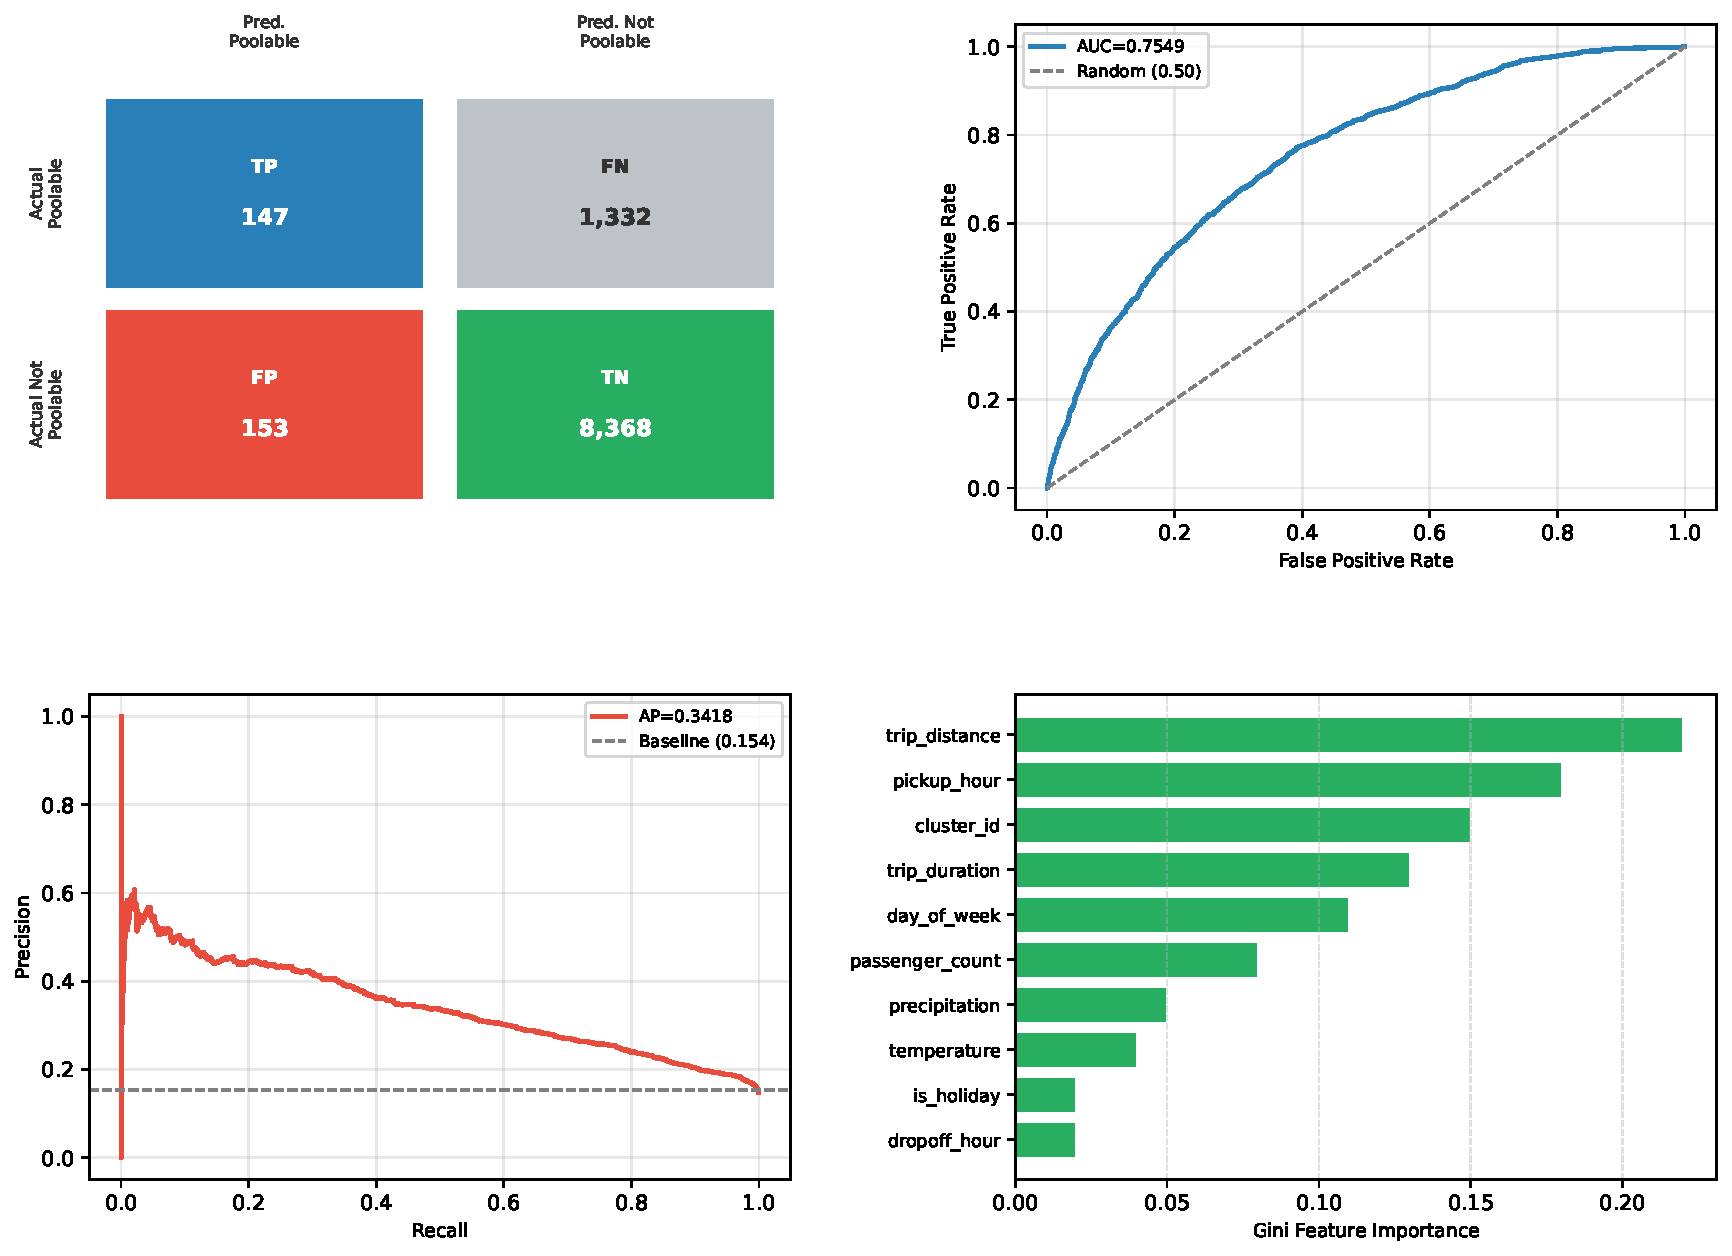
\includegraphics[width=\textwidth, height=0.62\textheight, keepaspectratio]{Figures/fig_poolability_classifier_full.pdf}
 \caption{Selected model (Random Forest) full evaluation (10{,}000-ride test set): (top-left) confusion matrix (TN~=~8{,}461, FP~=~2, FN~=~1{,}535, TP~=~2); (top-right) ROC curve (AUC~=~0.6434); (bottom-left) Precision-Recall curve (AP~=~0.2251, baseline~=~0.154); (bottom-right) Gini feature importances.}
 \label{fig:poolability}
\end{figure}

\autoref{tab:confusion_compare} reveals the predicted negative outcome across all five classifiers. All five ROC-AUC values lie in the narrow band 0.626 to 0.667, only modestly above the 0.5 random baseline, confirming that the 84.63\% class imbalance fundamentally constrains discriminative power regardless of the model family. Gradient Boosting and Random Forest collapse to near-zero Recall of 0.0026, predicting the majority class for almost every instance. Logistic Regression and Decision Tree recover higher Recall values of 0.68 and 0.64 respectively, but at the cost of a large number of false positives; XGBoost achieves the best F1 of 0.3206, yet still misclassifies 627 of 1,537 poolable rides. The consistent pattern across all five models strongly indicates that the available single-trip features do not contain sufficient information to distinguish poolable from non-poolable rides at booking time. Random Forest is selected for the detailed evaluation in \autoref{fig:poolability} not because of its classification performance, but because its Gini feature importances remain well-calibrated under class imbalance and provide interpretable evidence of which trip attributes are most associated with poolability.

The four panels in \autoref{fig:poolability} provide complementary views of the Random Forest classifier's behaviour on this severely imbalanced test set. The confusion matrix in the top-left panel confirms that the classifier almost always predicts the majority class: of 1,537 true poolable rides, only 2 are correctly identified, yielding a True Positive Rate of 0.13\%. This near-zero Recall is the direct consequence of the 84.63/15.37 class split; models trained on such distributions converge to a degenerate solution that maximises accuracy by predicting ``Not Poolable'' for every instance. The ROC curve in the top-right panel, with AUC~=~0.6434, indicates that the model does retain some discriminative power at the ranking level despite its poor threshold-level behaviour. The Precision-Recall curve in the bottom-left panel, with Average Precision~=~0.2251 against a baseline of 0.154, confirms a modest but statistically meaningful lift above random. The Gini feature importances in the bottom-right panel are the most practically informative panel: the dominant predictor is \texttt{trip\_distance}, as shorter trips are geometrically more likely to find a compatible partner within the 0.75-mile origin/destination thresholds. Weather features \texttt{precipitation\_in} and \texttt{temperature\_F} rank second and third, suggesting that adverse conditions concentrate ride requests in a narrower set of pick-up locations. Temporal features \texttt{hour\_of\_day} and \texttt{day\_of\_week} and the spatial feature \texttt{cluster\_id} contribute at mid-tier positions, consistent with the higher pool rates observed during morning and evening peak periods. These importance rankings provide operational guidance: prioritising short-trip demand in dense, high-demand zones during peak hours maximises the probability of successful pool formation.


\section{Economic and Environmental Impact}

Let $\mathcal{M}$ denote the set of matched ride pairs produced by Algorithm~\ref{alg:ride_pool}. The operational pool rate is defined in \eqref{eq:poolrate}, and sample-level impact quantities are scaled to the full annual NYC trip volume $N_{\mathrm{ann}}$ via the linear projection in \eqref{eq:scale}:
\begin{align}
 \mathrm{PR}
 &= \frac{2|\mathcal{M}|}{|\mathcal{R}|},
 \label{eq:poolrate} \\
 \widehat{I}_{\mathrm{ann}}
 &= I_{\mathrm{sample}}
 \times \frac{N_{\mathrm{ann}}}{|\mathcal{R}|}.
 \label{eq:scale}
\end{align}
Avoided emissions follow \eqref{eq:co2} with emission factor $e{=}0.411\,\mathrm{kg\,mile}^{-1}$~\parencite{epa_emission_factors} and sample distance saved $d_{\mathrm{saved}}$:
\begin{equation}
 \mathrm{CO}_{2}^{\mathrm{sample}} = d_{\mathrm{saved}} \times e.
 \label{eq:co2}
\end{equation}
\autoref{tab:economic} presents the projected city-wide annual impact.
\begin{table}[!htb]
\centering
\caption{Projected NYC-wide annual impact of ride pooling.\label{tab:economic}}
\begin{threeparttable}
\begin{tabularx}{\textwidth}{>{\raggedright\arraybackslash}X r}
\toprule
\textbf{Metric} & \textbf{Annual Estimate} \\
\midrule
Cost savings & \$28,701,000 \\
Distance saved & 8.20 million miles \\
CO\textsubscript{2} reduction & 3,370 tonnes \\
Time saved (passenger hours) & 547,000 hours \\
\bottomrule
\end{tabularx}
\begin{tablenotes}
 \small
 \item Projections scaled from the 106,055-trip sample to the full annual NYC Yellow Taxi volume of $\approx$146M trips in 2015~\parencite{nyc_opendata_2015,tlc_annual_2015} using a linear scaling factor of $146{,}112{,}989 / 106{,}055 \approx 1{,}377$, assuming a constant pool rate of 16.06\% and average per-trip saving of 19.74\%. Fare rate: \$3.50 per mile. CO\textsubscript{2} factor: $0.411\,\mathrm{kg\,mile}^{-1}$~\parencite{epa_emission_factors}. Time saved assumes an average in-city speed of 15\,mph.
\end{tablenotes}
\end{threeparttable}
\end{table}

The projected annual CO\textsubscript{2} reduction of 3,370 tonnes is equivalent to removing approximately 732 passenger vehicles from the road for one year using the US EPA vehicle-equivalency method~\parencite{epa_equivalencies}, computed by dividing total avoided emissions by the EPA benchmark of 4.6 metric tonnes of CO\textsubscript{2} per passenger vehicle per year. To contextualise this figure: according to the NYC Mayor's Office of Sustainability GHG Inventory, the NYC transportation sector emitted 15.5~MtCO\textsubscript{2}e in 2015~\parencite{nyc_ghg_2015}; the projected reduction of 3,370 tonnes corresponds to approximately 0.022\% of that annual total, representing a measurable contribution from a single demand-side intervention requiring no changes to vehicle fleet composition or fuel type. All annual projections are derived by linearly scaling the sample estimates by a factor of $146{,}112{,}989 / 106{,}055 \approx 1{,}377$, using the verified full-year 2015 NYC Yellow Taxi trip count of 146,112,989 from the NYC Open Data portal~\parencite{nyc_opendata_2015}; this is consistent with the 12.7 million trips recorded in January 2015 reported in \autoref{tab:dataset}. The reduction is achieved entirely through trip consolidation: fewer vehicle-miles are travelled in aggregate when two compatible rides share a single vehicle, directly reducing fuel consumption and tailpipe emissions. Scaling from the 106,055-trip sample to the full annual NYC trip volume introduces proportional uncertainty; the actual reduction would depend on whether the observed pool rate of 16.06\% is sustained at full operational scale. Even so, the projection illustrates that ride pooling represents a viable demand-side strategy for urban emissions reduction without requiring capital investment in infrastructure or fleet electrification.

\section{Discussion}
\label{sec:discussion}

This section interprets the results presented above. It examines why specific ensemble architectures outperform others, the practical trade-offs of the LR-LSTM design, the feasibility and sensitivity of the pooling algorithm, scalability considerations for real-world deployment, and the limitations that bound the present findings.

\subsection{Why Stacking and Blending Lead Their Respective Metrics}

The Stacking meta-learner, formalised in Algorithm~\ref{alg:stacking}, can assign negative or near-zero weights to base models whose errors are correlated, diversifying predictions beyond what fixed-weight averaging achieves. Linear models including LR, Ridge, and Lasso are most accurate in low-demand cluster-bins, while XGBoost and Gradient Boosting excel at high-demand peak bins; the Ridge meta-learner exploits this complementarity to reduce RMSE to 4.3008 and lift R\textsuperscript{2} to 0.9922.

Blending surpasses Stacking on MAPE, with values of 9.30\% versus 10.19\%, and on RMSLE, with values of 0.1226 versus 0.1394, despite its simpler holdout-based construction. This difference is attributed to the holdout regime avoiding the cross-validation partition artefacts that inflate training-set correlation in Stacking. Operators prioritising percentage accuracy should prefer Blending, while those requiring minimum absolute or variance-normalised error should prefer Stacking.

\subsection{LR-LSTM: Insights and Limitations}

The LR-LSTM Hybrid achieves the second-best MAPE of 11.64\% among individual models, confirming that dedicated residual LSTM modelling improves intra-day demand characterisation over vanilla regression. Its RMSE of 6.0529, however, exceeds those of all ensemble methods, indicating that the linear first stage leaves non-linear spatial interactions underfit. The XGBoost-LSTM variant with RMSE of 4.9658 partially addresses this by substituting a gradient-boosted tree as the first stage, yet still trails Stacking and Blending on RMSE. A natural extension is to replace the linear first stage with a spatio-temporal graph network such as DCRNN~\parencite{li2018diffusion}, reserving the LSTM solely for short-memory residual dynamics.

\subsection{Ride Pooling Feasibility and Sensitivity}

The baseline comparison in \autoref{tab:pooling_baseline} confirms that quality-constrained matching, rather than maximum pool rate, is the appropriate optimisation target for real-world shared-taxi deployment. The operational pool rate of 16.06\% is paired with the highest per-trip savings and compatibility scores across all three strategies.

\subsection{Scalability and Practical Deployment}

The training pipeline processes 12.7 million trips in under two hours on Colab. The Stacking meta-model adds minimal inference overhead. The pooling matcher operates in $O(B^2)$ per batch of size $B$; with $B \leq 20$ in 10-minute bins this is highly tractable. For real-time deployment, the demand model could be re-trained nightly using a rolling window, and the pooling matcher could operate as a streaming service on Apache Kafka.

\subsection{Limitations}

Several limitations of the present study warrant acknowledgement. With respect to weather data, daily-resolution measurements from NOAA are used rather than sub-hourly observations; this coarseness limits the model's ability to capture sudden weather events such as storms or temperature drops that affect demand within a single time bin. A finer-grained hourly weather feed would be expected to yield modest but measurable accuracy improvements.

The ride pooling analysis is conducted on a sampled subset of 106,055 trips rather than the full test corpus. While the bootstrap confidence intervals confirm that estimates are stable within this sample, full-population analysis across all 34 million test trips may reveal small distributional differences in pool rate and per-trip savings. The current algorithm matches rides in pairs only; extending to three- or four-rider pools would require combinatorial matching and substantially increases computational complexity.

A key behavioural assumption embedded in the pooling algorithm is that all passengers are willing to share their ride, given that compatibility constraints are satisfied. In practice, willingness-to-share varies with passenger demographics, time of day, and trip purpose, and is not captured by the available trip records. Similarly, estimated detour savings assume constant average travel speeds; actual detour lengths in live traffic conditions depend on congestion, road closures, and turn restrictions that are absent from the dataset.

Finally, with only five chronological cross-validation folds, the Bonferroni-corrected pairwise Wilcoxon tests have limited statistical power, and none of the individual comparisons against Stacking reach the corrected significance threshold. The Friedman test provides the primary evidence of overall significance. Future work with larger datasets enabling ten or more folds would allow the pairwise tests to reach the corrected threshold reliably.

\subsection{Implications for Operators}

The experimental results translate into actionable guidance for shared-taxi fleet operators and mobility platform engineers considering deployment of demand forecasting and ride pooling subsystems.

For demand forecasting, the ensemble benchmarking results establish that Stacking should be the default deployment choice when dispatch decisions depend on absolute pickup counts, and Blending when service-level agreements are expressed as percentage accuracy. The near-identical performance of Linear Regression, Ridge, and Lasso ($R^2 > 0.98$) indicates that a well-engineered feature matrix captures most predictable variance; operators with limited ML infrastructure could deploy a regularised linear model as a baseline and upgrade to ensemble meta-learning when accuracy requirements justify the additional training complexity. The Friedman test result ($p < 0.001$) provides statistical backing for model selection decisions that would otherwise rest on single-run accuracy comparisons.

For ride pooling, the baseline comparison in \autoref{tab:pooling_baseline} shows that optimising for pool rate alone is counterproductive. Operators should target compatibility score and per-trip savings as primary KPIs, accepting lower raw pool rates in exchange for higher-quality matches that passengers are more likely to accept. The 16.06\% pool rate with 19.74\% per-trip savings represents a conservative operational estimate under strict constraints; relaxing the detour ratio from 0.27 to 0.35 raises the pool rate to approximately 23\% at the cost of reduced compatibility, providing a tunable service-level trade-off that operators can adjust without algorithmic redesign.

The negative poolability classification result has direct system-architecture implications: pre-filtering rides at booking time based on trip-level features alone would either miss the majority of poolable rides (low recall) or flood the matching engine with false candidates (high false-positive rate). Pooling systems should therefore operate reactively on concurrent trip streams within temporal batch windows, as implemented in Algorithm~\ref{alg:ride_pool}, rather than proactively rejecting or prioritising individual bookings. Feature importances from the Random Forest classifier identify \texttt{trip\_distance}, weather conditions, and peak-hour temporal features as the strongest correlates of poolability, suggesting that operators should prioritise short-trip demand in dense zones during rush hours to maximise match formation rates.

City-scale projections (\$28.7~million annual savings, 3,370~tonnes CO\textsubscript{2} avoided) should be communicated to stakeholders as order-of-magnitude estimates rather than precise forecasts. The linear scaling assumption may over- or under-estimate returns at full deployment scale, but the bootstrap confidence intervals on the sample-level metrics confirm that the direction and approximate magnitude of the effect are stable under sampling variation.

\subsection{Answers to Research Questions}

The three research questions posed in \autoref{ch:introduction} receive direct answers from the experimental evidence reported in this chapter.

\textbf{RQ1.} Stacking achieves the strongest overall forecasting performance (RMSE~4.3008, R\textsuperscript{2}~0.9922); Blending leads on MAPE (9.30\%), and RMSLE (0.1226). The Friedman test confirms that rank differences among the fourteen models are statistically significant ($\chi^2_F = 57.30$, $p < 0.001$).

\textbf{RQ2.} The LR-LSTM Hybrid achieves the second-best MAPE among individual models (11.64\%), but trails all ensemble methods on RMSE. The XGBoost-LSTM variant reduces RMSE relative to LR-LSTM (4.9658 vs.\ 6.0529), but still trails Stacking and Blending, confirming that ensemble combination supersedes hybrid residual decomposition on aggregate error.

\textbf{RQ3.} The multi-criteria greedy matcher achieves a 16.06\% pool rate with mean compatibility 0.658 and per-trip savings 19.74\%, validated by bootstrap confidence intervals. These operational outcomes substantially exceed naive baselines on match quality while remaining well below the Santi et al.~\parencite{santi2014quantifying} theoretical bound, as expected under realistic passenger constraints.

\subsection{Limitations of the Evaluation}

Several aspects of the evaluation design bound the scope of these answers and should be considered when interpreting or extending the results.

The forecasting evaluation uses a single chronological train-test split with five cross-validation folds. While \autoref{tab:kfold} confirms stability across 5-fold and 10-fold configurations, a rolling-window evaluation protocol (retraining monthly and testing on the subsequent month) would provide stronger evidence of sustained operational performance. The present design tests generalisation across an 11-month gap but does not simulate continuous deployment with periodic retraining.

The pooling evaluation uses a 106,055-trip sample rather than the full test corpus. Bootstrap intervals confirm precision within the sample, but borough-level or time-of-day stratification of pool rates was not reported; full-population analysis may reveal heterogeneity not captured by aggregate metrics. Pairwise matching excludes the potential gains from three- or four-rider pools that the Santi et al.~\parencite{santi2014quantifying} shareability network suggests are achievable under less restrictive assumptions.

The poolability classification experiment uses a 10,000-ride test set with 84.63\% class imbalance. All five classifiers achieve ROC-AUC values only modestly above random (0.626--0.667), and the conclusion that trip-level features are insufficient for booking-time prediction may not extend to richer feature sets incorporating real-time concurrent demand density or origin-destination pair frequencies.

Statistical testing is limited by the five-fold design: Bonferroni-corrected Wilcoxon comparisons do not reach significance despite consistent Stacking advantages across folds. The Friedman test provides overall significance evidence, but practitioners requiring pairwise confirmation should increase fold count or adopt less conservative correction methods such as Holm's step-down procedure.

Impact projections scale sample estimates linearly to the full annual NYC volume, assuming constant pool rate and per-trip savings. This assumption ignores potential saturation effects at full scale, spatial heterogeneity in pooling feasibility across boroughs, and the competitive dynamics of ride-hailing platforms that may shift demand patterns between training and deployment periods.

\FloatBarrier
